\documentclass{beamer}

\usepackage{graphicx}
\usepackage{amssymb}
\usepackage{framed}
\usepackage{subfiles}
\begin{document}
%-------------------------------------------- %
% Schedule 0 
% Leadout
% - PyData Berlin and London
% Schdule 1
%  - Anaconda
%  - Building Bloack - numpy pandas etc
% Schedule 2 
%  - SKL capabilities
%============================================ %
\begin{frame}
	\huge
	
	\[\mbox{Introduction to Machine Learning} \]
	\[\mbox{with scikit.learn}\]
	\bigskip
	\[ \mbox{West of Ireland Data Science} \]
\end{frame}
%============================================ %
\begin{frame}[fragile]
	\frametitle{scikit.learn - Machine Learning with Python}
	\LARGE
	\begin{itemize}
		\item Some Opening Comments
		\item Python Environment
		\item What is Machine Learning?
		\item Scikit-Learn
		\item Classification with Scikit-Learn
	\end{itemize}
	
\end{frame}
\subfile{00-leadout.tex}
\subfile{01-Introduction.tex}

%============================================ %	
\subfile{02-machinelearning}
%=========================================================== %
\begin{frame}
	\begin{figure}
		\centering
		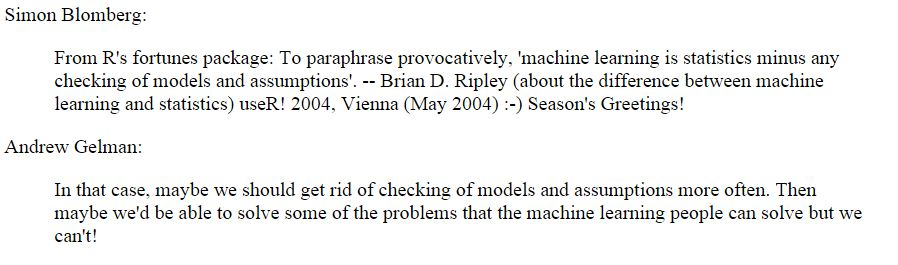
\includegraphics[width=1.1\linewidth]{machinelearningquotes}
	\end{figure}
	\Large Machine Learning is statistics minus any checking of models or assumptions
\end{frame}
%============================%
\begin{frame}
	\frametitle{The Data Science Profession}
	Data Science Retreat (Berlin)
	\begin{quote}
		MOOC have not  decreased the barrier of entry to machine-learning.
		
		
		Nowadays, you cannot be 'the guy who knows how to run (insert off-the-shelf-algo-here)'. 
		
		
		In dataland, that's the equivalent to being a code monkey. MOOCs and superb libraries (scikit-learn, R's ecosystem) made 
		sure there is plenty of people who can throw say a random forest to a problem. In the modern world, this is not adding that much value. 
	\end{quote}
\end{frame}
%===========================================================%

\begin{frame}
	\frametitle{scikit.learn}
	\begin{figure}
		\centering
		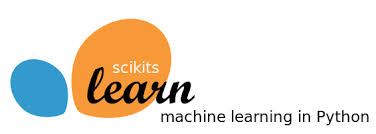
\includegraphics[width=0.5\linewidth]{SKL-logo2}
		
	\end{figure}
	
	\begin{itemize}
		\item scikit-learn is an open source machine learning library for the Python programming language. 
		\item scikit-learn features various classification, regression and clustering algorithms including support vector machines, logistic regression, naive Bayes, random forests, gradient boosting, k-means and DBSCAN. \item scikit-learn is designed to interoperate with the Python numerical and scientific libraries NumPy and SciPy.
	\end{itemize}
\end{frame}
%===========================================================%
\begin{frame}
	\textbf{Sci-Kit Learn Site info}
	\begin{figure}
		\centering
		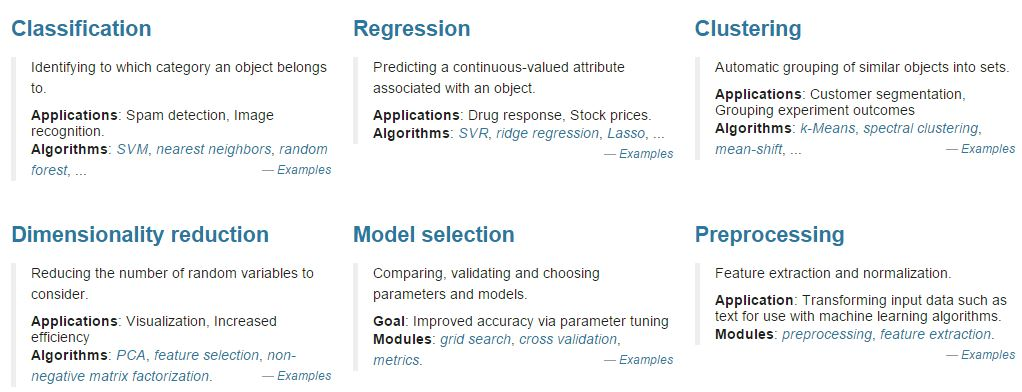
\includegraphics[width=1.1\linewidth]{SKLsiteinfo}
	\end{figure}
\end{frame}
%===========================================================%
\begin{frame}
	\begin{figure}
		\centering
		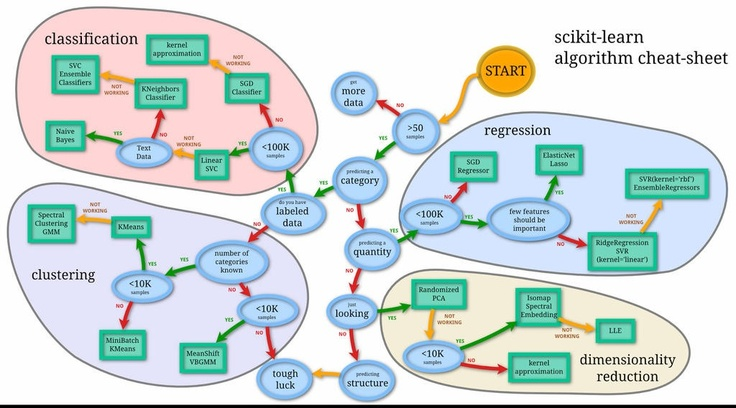
\includegraphics[width=0.9\linewidth]{SKLCheatSheet}
		
	\end{figure}
\end{frame}
%===========================================================%
\begin{frame}
	\begin{figure}
		\centering
		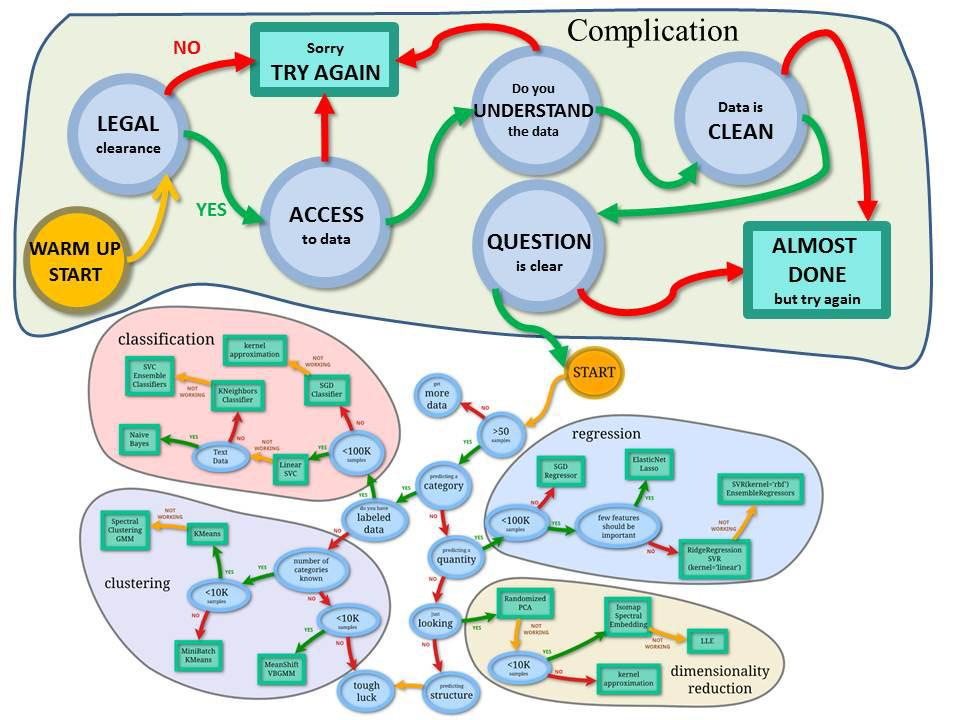
\includegraphics[width=0.9\linewidth]{SKLCheatSheet2}
		
	\end{figure}
\end{frame}

\subfile{02-skltopics.tex}
\subfile{07-sklclass.tex}
\subfile{03-decisiontrees.tex}
\subfile{03-SVMs.tex}

%============================================ %
\begin{frame}[fragile]
\frametitle{scikit.learn - Machine Learning with Python}
\LARGE	
\begin{framed}
\begin{verbatim}
import scikit.learn
\end{verbatim}
\end{framed}
\end{frame}
%============================================ %	


\end{document}
